% chap3_factoid.tex
%

\mychapter{Combining Data Sources for Factoid Question Answering}
\label{chapter:factoid}

\noindent

The majority of user web searches are entity-centric, \ie looking for some information or wanting to transact (\eg buy, download) on entities~\cite{pound2010ad}.
Questions that are asking about certain entities (\eg person, movie, product \etc) or their attributes (\eg date or number) are usually referred to as factoid questions.
This section describes the problem I'm going to focus on in my thesis, some existing results and proposals for future research.

\section{Problem}
\label{section:factoid:problem}

Factual information exists in many various formats: natural language statements, tables, question-answer (QnA) pairs, structured databases (DB) and knowledge bases (KB), images and other multimedia resources, \etc
Information stored in these data sources can be very useful to solve diverse user information tasks.
Moreover, due to different nature of the data sources, their pros and cons are often complimentary, and therefore their combination would have a synergistic effect.
In particular, text document collections~\cite{Kolomiyets:2011:SQA:2046840.2047162} and structured knowledge bases~\cite{unger2014introduction} are very useful for automatic factoid question answering.
For example, natural language text is relatively easy to match against user questions, especially given the redundancy of the information in large text collections, such as the web~\cite{lin2007exploration}.
On the contrary, for knowledge bases, translating a question into one of the structured query languages can be very challenging~\cite{BerantCFL13:sempre}.
Moreover, text encodes all kinds of factual knowledge, whereas knowledge base schemes are often very limited, and a set of objects, predicates and facts are often far from being complete~\cite{Dong:2014:KVW:2623330.2623623}.
According to D.Wimalasuriya and D.Dou~\cite{wimalasuriya2010ontology}, about 80\% of information contained in business documents is stated in natural language, \ie unstructured format.
However, text fragments include very limited amount of information about the mentioned entities, which complicates the reasoning and often require certain prediction models to be built~\cite{LiRoth02}.
Knowledge bases on the other hand aggregate all the information around entities and allow very complicated queries using special languages such as SPARQL.
Therefore, an idea to combine unstructured text and structured knowledge bases for joint question answering is very appealing and some existing research demonstrated its potential~\cite{elbassuoni2009language,fader2013paraphrase,ferrucci2010building,Sun:2015:ODQ:2736277.2741651,baudivs2015yodaqa}.
Prior approaches to the problem of combining textual and structured knowledge base data either process data sources using separate pipelines and merge the results~\cite{ferrucci2010building,baudivs2015yodaqa}, extract structured knowledge from text~\cite{Agichtein:2000:SER:336597.336644,MintzBSJ09,Dong:2014:KVW:2623330.2623623}, convert both data sources into a semi-structured format~\cite{Fader:2014:OQA:2623330.2623677}, extend knowledge bases with information extracted from text~\cite{elbassuoni2009language,yahya2016question} or 
enrich text with some knowledge about the mentioned entities~\cite{Sun:2015:ODQ:2736277.2741651}.
Unfortunately, such approaches usually sacrifices some potentially useful information available in the data sources.
For example, relation extraction methods extract only a small fraction of information encoded in text documents~\cite{Dong:2014:KVW:2623330.2623623}, and existing models of semantic enrichment of text data only uses a subset of KB~\cite{Sun:2015:ODQ:2736277.2741651}.

In summary, in my thesis I'm focusing on the problem of combining information available in textual data sources and structured knowledge bases to improve factoid question answering.
The focus of the proposed research is on utilizing all the available information of different data sources for joint reasoning.

\section{Approaches}
\label{section:factoid:approaches}

This section describes my previous research on the problem, \ie relation extraction from question-answer pairs (Section~\ref{section:factoid:approaches:cqarelextract}) and using external textual data to improve knowledge base question answering (Section~\ref{section:factoid:approaches:text2kb}).

% =-=-=-=-=-=-=-=-=-=-Cqa Relation Extraction: Begin-=-=-=-=-=-=-=-=-=-=-=-=-=-=-

\subsection{Relation Extraction from Question-Answer Pairs}
\label{section:factoid:approaches:cqarelextract}

Knowledge Bases were found to be quite effective in answering some of the users factual information needs \cite{unger2014introduction}.
However, KBs are inherently incomplete, \ie a lot of information is simply missing even from the largest existing knowledge bases.
According to Dong et al~\cite{Dong:2014:KVW:2623330.2623623}, 71\% of people in
Freebase have no known place of birth, and 75\% have no known nationality.
One approach to bridge this knowledge gap is automatic knowledge extraction from other data sources, \eg natural language sentence \cite{Agichtein:2000:SER:336597.336644,Gupta:2014:BOS:2732286.2732288,jijkoun2004information,MintzBSJ09}, tables \cite{Cafarella:2008:WEP:1453856.1453916}, \etc
In this section I focus on yet another source of information: question-answer pairs.

CQA websites, such as Yahoo! Answers\footnote{http://answers.yahoo.com/}, Answers.com\footnote{http://www.answers.com}, Quora\footnote{http://quora.com} \etc, has gained a lot of popularity in the recent years, and their archives store hundreds of millions of user questions along with answers provided by the community.
Many users' information needs are not unique and arise again and again, which makes it possible to reuse the information to answers new questions \cite{Shtok:2012:LPA:2187836.2187939}.
This idea makes CQA data attractive for knowledge base population.
Although some of the facts mentioned in QnA pairs can also be found in some other text documents, another part might be unique (\eg in Clueweb\footnote{http://www.lemurproject.org/clueweb12/} about 10\% of entity pairs with existing Freebase relations mentioned in Yahoo! Answers documents cannot be found in other documents \cite{savenkov2015relation}).
Existing relation extraction techniques face some challenges when applied to CQA data, \ie they typically consider sentences independently and ignore the discourse of a QnA pair text.
However, frequently, it is impossible to understand the answer without knowing the question.
For example, sometimes users simply give the answer to the question without stating it in a narrative sentence (\eg ``\emph{What does "xoxo" stand for? Hugs and kisses.}``), or the provided answer might contain ellipsis, \ie some important information is omitted (\eg ``\emph{What's the capital city of Bolivia? Sucre is the legal capital, though the government sits in La Paz}``).

In my thesis I propose a novel model for relation extraction from CQA data, that uses discourse of a QnA pair to extract facts between entities mentioned in question and answer sentences.
The conducted experiments confirm that many of such facts cannot be extracted by existing sentence-based techniques and thus it is beneficial to combine their outputs with the output of our model.

More formally, the target problem is relation extraction from QnA data, which is a collection of $(q, a)$ pairs, where $q$ is a question text (can contain multiple sentences) and $a$ is the corresponding answer text (can also contain multiple sentences).
By relation instance $r$ we mean an ordered binary relation between $subject$ and $object$ entities, which is commonly represented as $[subject, predicate, object]$ triple.
For example, the fact that Brad Pitt married Angelina Jolie can be represented as [Brad Pitt, married\_to, Angelina Jolie].
In this work we use Freebase, an open schema-based KB, where all entities and predicates come from the fixed alphabets $E$ and $P$ correspondingly.
Let $e_1$ and $e_2$ be entities that are mentioned together in a text (\eg in a sentence, or $e_1$ in a question and $e_2$ in the corresponding answer), we will call such an entity pair with the corresponding context a mention.
The same pair of entities can be mentioned multiple times within the corpus, and for all mentions $i=1,...,n$ the goal is to predict the expressed predicate ($z_i \in P$) or to say that none applies ($z_i = \emptyset$).
Individual mention predictions $z_1, ..., z_n$ are combined to infer a set of relations $\mathbf{y}=\{y_i \in P\}$ between the entities $e_1$ and $e_2$.

\begin{figure}[h]
\centering
\begin{tikzpicture}
\tikzstyle{main}=[circle, minimum size = 8mm, thick, draw =black!80, node distance = 14mm]
\tikzstyle{mainnob}=[circle, minimum size = 8mm, thick, draw =white!100, node distance = 14mm]
\tikzstyle{connect}=[-latex, thick]
\tikzstyle{box}=[rectangle, draw=black!100]
\node[main, fill = white!100] (y) [label=center:$y$] { };
\node[rectangle, inner sep=-1mm, fit=(y),label=below right:$P$] {};
\node[rectangle, inner sep=4mm, fit=(y),draw=black!100] {};
\node[main, fill = white!100] (z) [below=of y,label=center:$z$] { };
%\node[rectangle, inner sep=-1mm, fit=(z),label=below right:$P$] {};
%\node[rectangle, inner sep=4mm, fit=(z),draw=black!100] {};
\node[main, fill = black!10] (x) [below=of z,label=center:$\mathbf{x}$] { }; 
\node[main, fill = black!10] (t) [right=of z,label=center:$\mathbf{x_t}$] { };
\node[mainnob, fill = white!100] (wt) [right=of y,label=center:$\mathbf{w_t}$] { };
\node[mainnob, fill = white!100] (wx) [left=of y,label=center:$\mathbf{w_x}$] { };
\node[rectangle, inner sep=-1mm, fit=(z)(x)(t),label=below right:$|Q|$, yshift=-1mm] {};
\node[rectangle, inner sep=6.5mm, fit=(z)(x)(t),draw=black!100] {};

\node[rectangle, inner sep=-1mm, fit=(z)(x),label=below right:$M$,yshift=-12mm] {};
\node[rectangle, inner sep=5.0mm, fit=(z)(x),draw=black!100] {};

\node[rectangle, inner sep=-1mm, fit=(x)(z)(y),label=below right:$N$,yshift=-30mm,xshift=4.5mm] {};
\node[rectangle, inner sep=9mm, fit=(x)(z)(y),draw=black!100, yshift=-3mm] {};

\path (wx) edge [connect] (z)
(x) edge [connect] (z)
(z) edge [connect] (y)
(wt) edge [connect] (z)
(t) edge [connect] (z);
\end{tikzpicture}
\caption{QnA-based relation extraction model plate diagram.
$N$ - number of different entity pairs, $M$ - number of mentions of an entity pair, $|Q|$ - number of questions where an entity pair is mentioned, $\mathbf{x}$ and $\mathbf{x_t}$ - mention-based and question-based features, $\mathbf{w}$ and $\mathbf{w_t}$ - corresponding feature weights, latent variables $z$ - relation expressed in an entity pair mention, latent variables $y$ - relations between entity pair}
\label{figure:qna_relextract:graphmodel}
\end{figure}

The proposed models for relation extraction from QnA data incorporates the topic of the question and can be represented as a graphical model (Figure \ref{figure:qna_relextract:graphmodel}).
Each mention of a pair of entities is represented with a set of mention-based features $x$ and question-based features $x_t$.
A multinomial latent variable $z$ represents a relation (or none) expressed in the mention and depends on the features and a set of weights $w_x$ for mention-based and $w_t$ for question-based features:
$$\hat{z}=\argmax{z \in P \cup \emptyset} p(z|x, x_t, w_x, w_t)$$.
To estimate this variable we use L2-regularized multinomial logistic regression model, trained using the distant supervision approach for relation extraction \cite{MintzBSJ09}, in which mentions of entity pairs related in Freebase are treated as positive instances for the corresponding predicates, and negative examples are sampled from mentions of entity pairs which are not related by any of the predicates of interest.
Finally, to predict a set of possible relations $\mathbf{y}$ between the pair of entities we take logical OR of individual mention variables $\mathbf{z}$, \ie $y_p = \lor_{i=1}^M [z_i = p, p \in P]$, where M is the number of mentions of this pair of entities.

\subsubsection{Sentence-based baseline model}
\label{section:factoid:approaches:cqarelextract:baseline}

Existing sentence-based relation extraction models can be applied to individual sentences of a QnA pair and will work well for complete statements, \eg ``Who did Brad Pitt marry? Brad Pitt and Angelina Jolie married at secret ceremony ...''.
In sentence-based scenario, when the set of question-based features is empty, the above model corresponds to the Mintz++ baseline described in \cite{Surdeanu:2012:MML:2390948.2391003}, which was shown to be superior to the original model of \cite{MintzBSJ09}, is easier to train than some other state of the art distant supervision models and produces comparable results.

\subsubsection{Sentence-based model with question features}
\label{section:factoid:approaches:cqarelextract:baselineqfeat}

\begin{table*}[tbh]
\centering
\begin{tabular}{|p{9cm}|p{7.8cm}|}
\hline
\multicolumn{2}{|c|}{Sentence-based model}\\
\hline
Dependency path between entities & \texttt{[PERSON]$\rightarrow$nsubjpass(born)tmod$\leftarrow$[DATE]}\\
Surface pattern & \texttt{[PERSON] be/VBD born/VBN [DATE]}\\
\hline
\hline
\multicolumn{2}{|c|}{Question features for sentence-based model}\\
\hline
Question template & \texttt{when [PERSON] born}\\
Dependecy path from a verb to the question word & \texttt{(when)$\rightarrow$advmod(born)}\\
Question word + dependency tree root & \texttt{when+born}\\
\hline
\hline
\multicolumn{2}{|c|}{QnA-based model}\\
\hline
Question template + answer entity type & \texttt{Q: when [PERSON] born A:[DATE]}\\
Dependency path from question word to entity & \texttt{Q:(when)$\rightarrow$advmod(born)nsubj$\leftarrow$[PERSON]}\\
and answer entity to the answer tree root & \texttt{A: (born)tmod$\leftarrow$[DATE]}\\
Question word, dependency root and answer pattern & \texttt{Q: when+born A:born [DATE]}\\
\hline
\end{tabular}
\caption{Examples of features used for relation extraction for ``\emph{When was Mariah Carey born? Mariah Carey was born 27 March 1970}''}
\label{table:qna_relextract:features}
\end{table*}

In many cases an answer statement is hard to interpret correctly without knowing the corresponding question.
To give the baseline model some knowledge about the question, we include question features (Table \ref{table:qna_relextract:features}), which are based on dependency tree and surface patterns of a question sentence. 
This information can help the model to account for the question topic and improve predictions in some ambiguous situations.

\subsubsection{QnA-based model}
\label{section:factoid:approaches:cqarelextract:qnamodel}

The QnA model for relation extraction is inspired by the observation, that often an answer sentence do not mention one of the entities at all, \eg, ``\textit{When was Isaac Newton born? December 25, 1642 Woolsthorpe, England}''.
To tackle this situation we make the following assumption about the discourse of a QnA pair: an entity mentioned in a question is related to entities in the corresponding answer and the context of both mentions can be used to infer the relation predicate.
Our QnA-based relation extraction model takes an entity from a question sentence and entity from the answer as a candidate relation mention, represents it with a set of features (Table \ref{table:qna_relextract:features}) and predicts a possible relation between them similar to sentence-based models.
The features are conjunctions of various dependency tree and surface patterns of question and answer sentences, designed to capture their topics and relation.

\subsubsection{Experiments}
\label{section:factoid:approaches:cqarelextract:experiments}

For experiments we used 2 publicly available CQA datasets: Yahoo! Answers WebScope dataset\footnote{http://webscope.sandbox.yahoo.com/catalog.php?datatype=l} and a crawl of WikiAnswers\footnote{http://wiki.answers.com/} collected by \cite{Fader:2014:OQA:2623330.2623677}.
The Yahoo! Answers dataset contains 4,483,032 questions (3,894,644 in English) with the corresponding answers collected on 10/25/2007.
The crawl of WikiAnswers has 30,370,994 question clusters, tagged by WikiAnswers users as paraphrases, and only 3,386,256 them have answers.
From these clusters we used all possible pairs of questions and corresponding answers (19,629,443 pairs in total).

\begin{table*}[ht]
\centering
\begin{tabular}{|p{12.5cm}||p{1.2cm}|p{1.2cm}|} \hline
& Y!A & WA\\
\hline
Number of QnA pairs & 3.8M & 19.6M \\
Average question length (in chars) & 56.67 & 47.03 \\
Average answer length (in chars) & 335.82 & 24.24 \\
% Number of resolved entities per QnA pair & 3.57 & 3.23 \\
Percent of QnA pairs with answers that do not have any verbs & 8.8\% & 18.9\% \\
Percent of QnA pairs with at least one pair of entities related in Freebase & 11.7\% & 27.5\% \\
Percent of relations between entity pairs in question sentences only & 1.6 \% & 3.1\% \\
Percent of relations between entity pairs in question and answer sentences only & 28.1\% & 46.4\% \\
Percent of relations between entity pairs in answer sentences only & 38.6\%& 12.0\%\\
\hline
\end{tabular}
\caption{Yahoo! Answers and WikiAnswers datasets statistics}
\label{table:qna_relextract:cqastats}
\end{table*}

For each QnA pair we applied tokenization, sentence detection, named entity tagger, parsing and coreference resolution from Stanford CoreNLP \cite{manning-EtAl:2014:P14-5}.
Our cascade entity linking approach is similar to \cite{chang2011stanford} and considered all noun phrase and named entity mentions as candidates.
First, all named entity mentions are looked up in Freebase names and aliases dictionary.
The next two stages attempt to match mention text with dictionary of English Wikipedia concepts \cite{spitkovsky2012cross} and its normalized version.
Finally for named entity mentions we try spelling correction using Freebase entity names dictionary.
We didn't disambiguate entities and instead took top-5 ids for each coreference cluster (using the $p(entity|phrase)$ score from the dictionary or number of existing Freebase triples).
All pairs of entities (or entity and date) in a QnA pair that are directly related\footnote{We also consider some paths that come through a mediator node, \eg  /people/person/spouse\_s./people/marriage/spouse} in Freebase were annotated with the corresponding relations.

Table \ref{table:qna_relextract:cqastats} gives some statistics on the datasets used in this work.
The analysis of answers that do not have any verbs show that $\sim$8.8\% of all QnA pairs do not state the predicate in the answer text.
The percentage is higher for WikiAnswers, which has shorter answers on average.
Unfortunately, for many QnA pairs we were unable to find relations between the mentioned entities (for many of them no or few entities were resolved to Freebase).
Among those QnA pairs, where some relation was annotated, we looked at the location of related entities.
In Yahoo! Answers dataset 38.6\% (12.0\% for WikiAnswers) of related entities are mentioned in answer sentences and can potentially be extracted by sentence-based model, and 28.1\% (46.4\% for WikiAnswers) between entities mentioned in question and answer sentences, which are not available to the baseline model and our goal is to extract some of them.

For our experiments we use a subset of 29 Freebase predicates that have enough unique instances annotated in our corpus, \eg date of birth, profession, nationality, education institution, date of death, disease symptoms and treatments, book author, artist album, \etc
We train and test the models on each dataset separately.
Each corpus is randomly split for training (75\%) and testing (25\%).
Knowledge base facts are also split into training and testing sets (50\% each).
QnA and sentence-based models predict labels for each entity pair mention, and we aggregate mention predictions by taking the maximum score for each predicate.
We do the same aggregation to produce a combination of QnA- and sentence-based models, \ie, all extractions produced by the models are combined and if there are multiple extractions of the same fact we take the maximum score as the final confidence.
The precision and recall of extractions are evaluated on a test set of Freebase triples, \ie an extracted triple is considered correct if it belongs to the test set of Freebase triples, which are not used for training (triples used for training are simply ignored).
Note, that this only provides a lower bound on the model performance as some of the predicted facts can be correct and simply missing in Freebase.

Figure \ref{figure:qna_relextract:pr_curve} shows Precision-Recall curves for QnA-based and sentence-based baseline models and some numeric results are given in Table \ref{table:qna_relextract:results}.
As 100\% recall we took all pairs of entities that can be extracted by either model.
It is important to note, that since some entity pairs occur exclusively inside the answer sentences and some in pairs of question and answer sentences, none of the individual models is capable of achieving 100\% recall, and maximum possible recalls for QnA- and sentence-based models are different.

\begin{figure}[h!]
\centering
\vspace{-2mm}
\begin{subfigure}[h]{0.45\textwidth}
	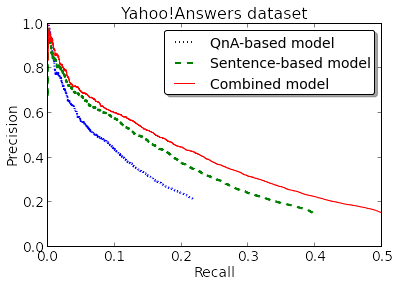
\includegraphics[width=0.99\textwidth]{img/cqarelextract_qa_vs_sent_ya}
	\vspace{-1mm}
    \label{figure:pr:ya}
\end{subfigure}
\begin{subfigure}[h]{0.45\textwidth}
	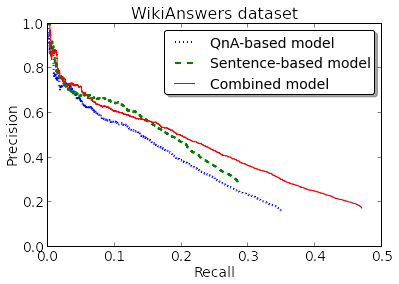
\includegraphics[width=0.99\textwidth]{img/cqarelextract_qa_vs_sent_wa}
	\vspace{-1mm}
    \label{figure:pr:wa}
\end{subfigure}
\begin{subfigure}[h]{0.45\textwidth}
	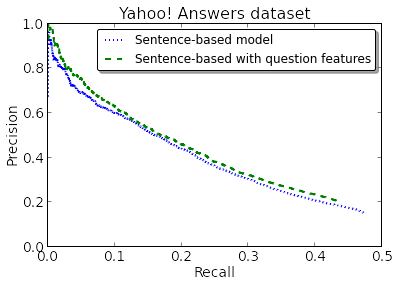
\includegraphics[width=0.99\textwidth]{img/cqarelextract_noqf_vs_qf}
	\vspace{-1mm}
	\label{figure:pr:noqf_vs_qf}
\end{subfigure}
\vspace{-1mm}
\caption{Precision-Recall curves for QnA-based vs sentence-based models and sentence-based model with and without question features}
\label{figure:qna_relextract:pr_curve}
\end{figure}

\begin{table*}[tbh]
\centering
\begin{tabular}{|p{6.6cm}||p{0.9cm}|p{1.4cm}|p{1.6cm}||p{0.9cm}|p{1.4cm}|p{1.6cm}|}
\hline
& \multicolumn{3}{|c||}{Yahoo! Answers} & \multicolumn{3}{|c|}{WikiAnswers}\\
\cline{2-7}
& QnA & Sentence & Combined & QnA & Sentence & Combined\\
\hline
F-1 score & 0.219 & 0.276 & 0.310 & 0.277 & 0.297 & 0.332\\
Number of correct extractions & 3229 & 5900 & 7428 & 2804 & 2288 & 3779 \\
Correct triples not extracted by other model & 20.5\% & 56.5\% & - & 39.4\% & 25.8\% & - \\
\hline
\end{tabular}
\caption{Extraction results for QnA- and sentence-based models on both datasets}
\label{table:qna_relextract:results}
\end{table*}

Results demonstrate that from 20.5\% to 39.4\% of correct triples extracted by the QnA-based model are not extracted by the baseline model, and the combination of both models is able to achieve higher precision and recall.
Unfortunately, comparison of sentence-based model with and without question-based features (Figure \ref{figure:qna_relextract:pr_curve}) didn't show a significant difference.

\subsubsection{Analysis}

To get an idea of typical problems of QnA-based model we sampled and manually judged extracted high confidence examples that are not present in Freebase (and thus are considered incorrect for precision-recall analysis).

The major reason (40\%) of false positive extractions is errors in entity linking.
For example: ``\emph{Who is Tim O'Brien? He was born in Austin on October 1, 1946}''.
The model was able to correctly extract [Tim O'Brien, date\_of\_birth, October 1, 1946], however Tim O'Brien was linked to a wrong person.
In a number of cases (16\%) our discourse model turns out to be too simple and fails for answers, that mention numerous additional information, \eg ``\emph{How old is Madonna really? ...Cher was born on 20 May 1946 which makes her older that Madonna...}''.
A possible solution would be to either restrict QnA-based model to cases when no additional information is present or design a better discourse model with deeper analysis of the answer sentence and its predicates and arguments.
Some mistakes are due to distant supervision errors, for example for the music.composition.composer predicate our model extracts singers as well as composers (which are in many cases the same).

Of course, there are a number of cases, when our extractions are indeed correct, but are either missing (33\%) or contradicting with Freebase (8\%).
An example of an extracted fact, that is missing in Freebase is ``\emph{Who is Wole Soyinka? He studied at the University College, Ibadan(1952-1954) and the University of Leeds (1954-1957)}'', and [Wole Soyinka, institution, University of Leeds] is currently not present in Freebase.
Contradictions with Freebase occur because of different precision levels (``pianist'' vs ``jazz pianist'', city vs county, \etc), different calendars used for dates or ``incorrect'' information provided by the user.
An example, when existing and extracted relation instance are different in precision is:``\emph{Who is Edward Van Vleck? Edward Van Vleck was a mathematician born in Middletown, Connecticut}'' we extract [Edward Van Vleck, place\_of\_birth, Middletown], however the Freebase currently has USA as his place of birth.

The problem of ``incorrect'' information provided in the answer is very interesting and worth special attention.
It has been studied in CQA research, \eg \cite{shah2010evaluating}, and an example of such QnA pair is: ``\emph{Who is Chandrababu Naidu? Nara Chandra Babu Naidu (born April 20, 1951)}''.
Other authoritative resources on the Web give April 20, 1950 as Chandrababu Naidu's date of birth.
This raises a question of trust to the provided answer and expertise of the answerer.
Many questions on CQA websites belong to the medical domain, \eg people asking advices on different health related topics.
How much we can trust the answers provided to extract them into the knowledge base?
We leave this question to the future work.

Finally, we have seen that only a small fraction of available QnA pairs were annotated with existing Freebase relations, which shows a possible limitation of Freebase schema.
A promising direction for future work is automatic extraction of new predicates, which users are interested in and which can be useful to answer more future questions.

\subsubsection{Summary}
\label{section:factoid:approaches:cqarelextract:summary}

In this section we described a model for relation extraction from QnA data, which is capable of predicting relations between entities mentioned in question and answer sentences.
We conducted experiments on 2 publicly available CQA datasets and showed that our model can extract triples not available to existing sentence-based techniques and can be effectively combined with them for better coverage of a knowledge base population system.

% =-=-=-=-=-=-=-=-=-=-Cqa Relation Extraction: End-=-=-=-=-=-=-=-=-=-=-=-=-=-=-

% =-=-=-=-=-=-=-=-=-=-=-=-=-=-Text2KB: Begin=-=-=-=-=-=-=-=-=-=-=-=-=-=-=-=-=-

\subsection{Text2KB: Knowledge Base Question Answering using External Text Data}
\label{section:factoid:approaches:text2kb}

Converting unstructured information into structured form by extracting knowledge from text suffers from certain quality losses.
Existing relation extraction tools aren't perfect, in particular due to recall losses a lot of information is left behind.
Moreover, extractions contain certain level of incorrect information due to precision losses.
These errors cap the upper bound on the question answering system performance.
In this section, I describe a novel factoid question answering system, that utilizes available textual resources to improve different stages of knowledge base question answering (KBQA).

KBQA systems must address three challenges, namely question entity identification (to anchor the query process); candidate answer generation; and candidate ranking.
We will show that these challenges can be alleviated by the appropriate use of external textual data.
Entity identification seeds the answer search process, and therefore the performance of the whole system greatly depends on this stage \cite{yao-scratch-qa-naacl2015}.
Question text is often quite short, may contain typos and other problems, that complicate entity linking.
Existing approaches are usually based on dictionaries that contain entity names, aliases and some other phrases, used to refer to the entities \cite{SPITKOVSKY12.266}.
These dictionaries are noisy and incomplete, \eg to answer the question \textit{``what year did tut became king?''} a system needs to detect a mention \textit{``tut''}, which refers to the entity \texttt{Tutankhamun}.
If a dictionary doesn't contain a mapping \textit{``tut''} $\rightarrow$ \texttt{Tutankhamun}, as happens for one of the state of the art systems, it will not be able to answer the question correctly.
Such less popular name variations are often used along with full names inside text documents, for example, to avoid repetitions.
Therefore, we propose to look into web search results to find variations of question entity names, which can be easier to link to a KB (Figure \ref{figure:text2kb:web_search_entitylink}).
This idea has been shown effective in entity linking for web search queries\footnote{http://web-ngram.research.microsoft.com/ERD2014/} \cite{SMAPH_ERD:2014}.

\begin{figure}[!ht]
\centering
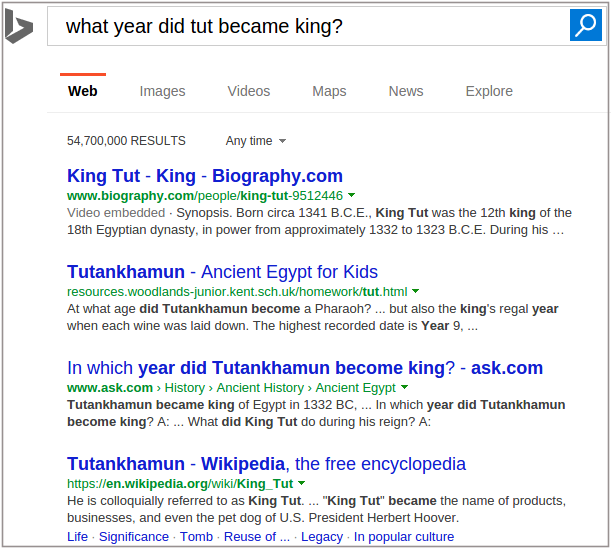
\includegraphics[width=0.5\textwidth]{img/web_search_entitylink}
\caption{Search results for the question \textit{``what year did tut became king?''}, which mention both the full name of the king and the correct answer to the question}
\label{figure:text2kb:web_search_entitylink}
\end{figure}

After question entities have been identified, answer candidates need to be generated and ranked to select the best answer.
A candidate query includes one or multiple triple patterns with predicates, corresponding to words and phrases in the question.
Existing knowledge base question answering approaches \cite{bastmore:cikm:2015:aquu,BerantCFL13:sempre,BerantL14:parasempre,berant2015imitation,BordesCW14:emnlp,yao2014freebase} rely on a lexicon, learned from manually labeled training data, and supported by additional resources, such as question paraphrases \cite{BerantL14:parasempre} and weakly labeled sentences from a large text collection \cite{YaoD14}.
Such training data tends to be small compared to the number of different predicates in a KB, and therefore the coverage of these lexicons is limited.
By our estimate, in a popular WebQuestions KBQA dataset~\cite{BerantCFL13:sempre}, the answers to $\sim$5.5\% of test questions (112 out of 2032) involve a predicate that does not appear as a ground truth in the training set.
For example, an RDF triple \texttt{[Bigos, food.dish.type\_of\_dish1, Stew]} answers the question \textit{``what are bigos?''}, but no other examples in the training set involve this predicate.
In addition, a lexicon needs to cover all different ways a predicate can be asked about.
For example, questions \textit{``who did jon gosselin cheat with?''} and \textit{``who is the woman that john edwards had an affair with?''} are answered by the same KB predicate, but use different language.
Therefore, presence of the first question in a training set may not help to answer the second question.
On the other hand, traditional Text-QA systems benefit from the redundancy of the information on the Web, where the same facts are stated multiple times in many different ways \cite{lin2007exploration}.
This increases the chances of a good lexical match between a question and answer statements, which makes even some relatively simple counting-based techniques quite effective \cite{brill2002analysis}.
We propose to adapt these ideas from text-based question answering for KBQA.

The general architecture and an example use case of Text2KB is presented on Figure \ref{figure:text2kb:model}.
Text2Kb is based on the information extraction approach to knowledge base question answering \cite{YaoD14}, in particular it extends the Aqqu system of H.Bast et al.~\cite{bastmore:cikm:2015:aquu}, which is one of the best performing open source KBQA system on the WebQuestions dataset.
The left part of the Figure \ref{figure:text2kb:model} describes a typical architecture of IE-based KBQA systems, and the right part introduces additional external text data sources, namely Web search results, community question answering (CQA) data, and a collection of documents with detected KB entity mentions.
First, we describe the main stages of the information extraction approach to knowledge base question answering using Aqqu, our baseline system, as an example.

\begin{figure*}[!ht]
\centering
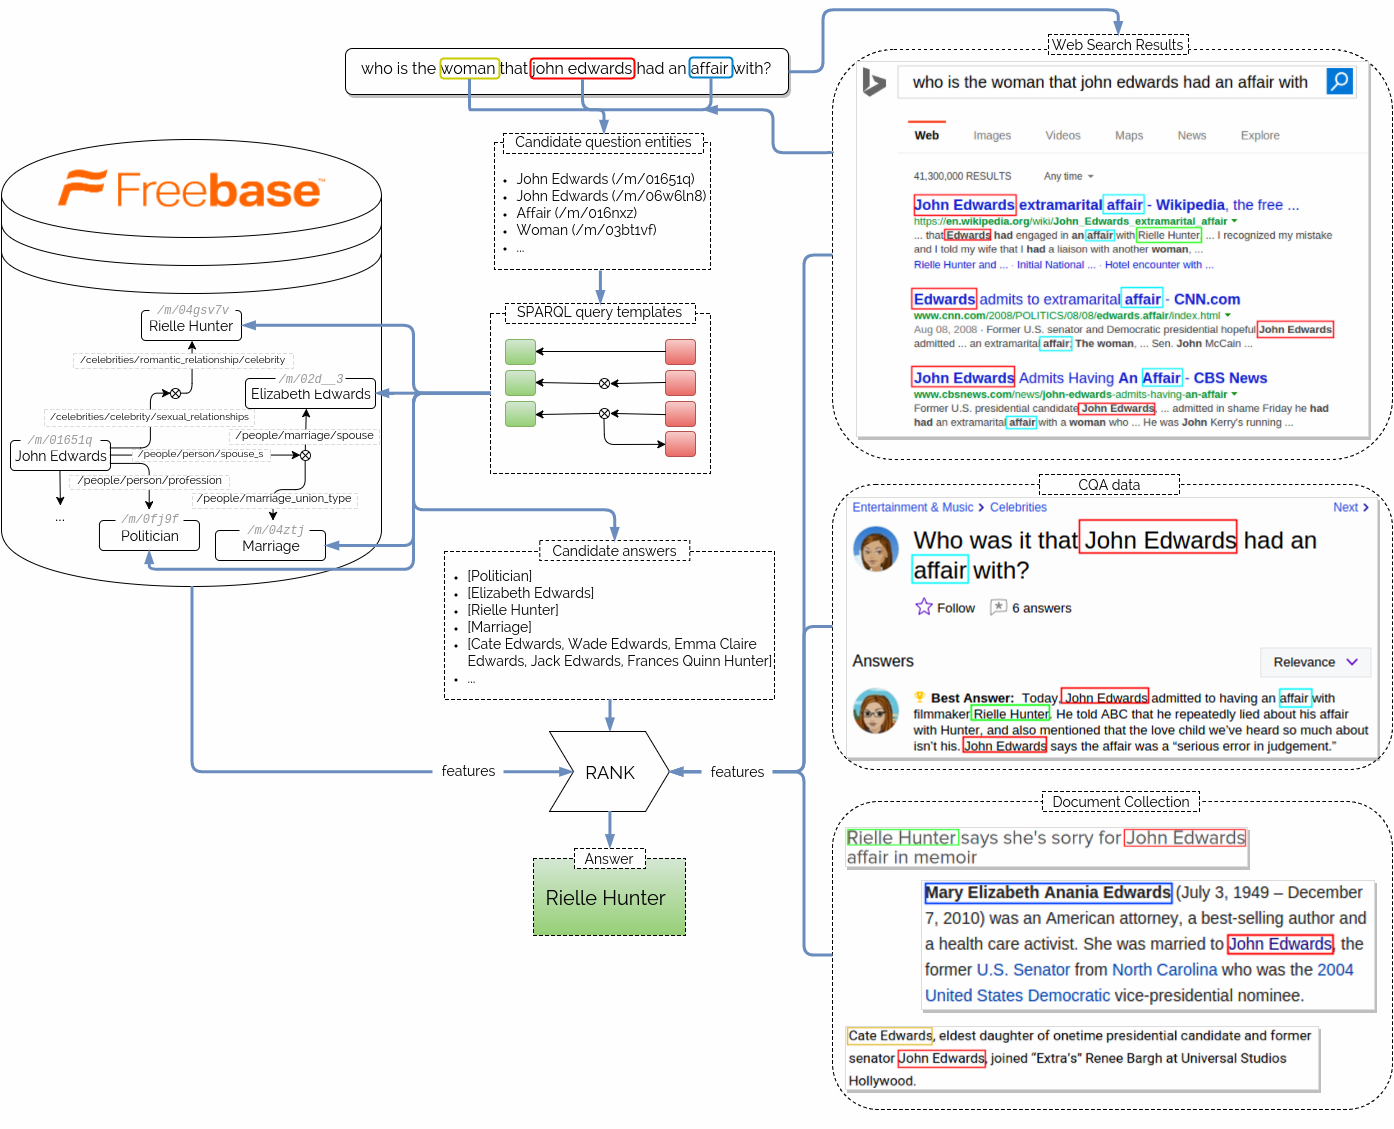
\includegraphics[width=\textwidth]{img/text2kb_model}
\caption{The architecture of our Text2KB Question Answering system}
\label{figure:text2kb:model}
\end{figure*}

\subsubsection{Information Extraction Approach to KBQA}
\label{section:factoid:approaches:text2kb:baseline}

The first stage of the knowledge base question answering process is identification of question topic entities, which are used as sources for the answer search process.
For concreteness, consider a question from the WebQuestions dataset \textit{``who is the woman that john edwards had an affair with?''}.
Here, the entity \texttt{John Edwards} with Freebase id \texttt{/m/01651q} is the main question entity.
However, Freebase contains millions of entities and it can be difficult to identify the topical ones (\eg entities \texttt{Woman} and \texttt{Affair} are also present in Freebase), or to disambiguate and choose between \texttt{John Edwards} a politician (\texttt{/m/01641q}), an American racing driver (\texttt{/m/06zs089}) and other people with the same name.
Aqqu considers all spans of question words under certain conditions on part of speech tags and uses an entity names lexicon \cite{SPITKOVSKY12.266} to map phrases to potential entities.
Most reported systems, including Aqqu, do not disambiguate entities at this stage, but rather keep a set of candidates along with some information about their popularities (\eg number of mentions in the collection), and mention scores $p(entity| mention\ text)$.

At the next stage, SPARQL query candidates are generated by exploring the neighborhood of the question topic entities using a predefined set of query templates.
Each query template has question entities, predicates and answer placeholders.
The majority of the answers in the WebQuestions dataset can be covered by just 3 templates (q\_entity - question entity, a\_entity - answer entity, cvt\_node - Freebase mediator node, which represent tuples with more than 2 arguments):
\\

\begin{lstlisting}[frame=single,basicstyle=\small]
SELECT DISTINCT ?a_entity {
   <q_entity> <predicate> ?a_entity .
}
\end{lstlisting}

\begin{lstlisting}[frame=single,basicstyle=\small]
SELECT DISTINCT ?a_entity {
   <q_entity> <predicate_1> ?cvt_node .
   ?cvt_node <predicate_2> ?a_entity .
}
\end{lstlisting}

\begin{lstlisting}[frame=single,basicstyle=\small]
SELECT DISTINCT ?a_entity {
   <q_entity_1> <predicate_1> ?cvt_node .
   ?cvt_node <predicate_2> <q_entity_2> .
   ?cvt_node <predicate_3> ?a_entity .
}
\end{lstlisting}

The first template retrieves a set of entities that are directly connected to the given question entity via a certain predicate.
The second template accounts for the presence of a mediator node, that groups together arguments of a multi-argument relation.
And the last template looks for cases, when a question also mentions another argument of a multi-argument relation, \eg \texttt{Captain Kirk} and \texttt{Star Trek} for the question \textit{``who played captain kirk in star trek movie?''}.

Each query candidate is represented with a set of features, that includes the scores for linked question entities, various scores for matching between question term n-grams and query predicates, the size of the results list, \etc
The final stage of the question answering process is filtering and ranking.
The Aqqu system employs a pairwise learning-to-rank model, trained on part of the dataset.
For each pair of candidate answers Aqqu creates an instance, which contains 3 groups of features: features of the first, the second candidate in the pair and the differences between the corresponding features of the candidates. Specifically, a Random Forest model is used in the provided Aqqu implementation. 
A pair where the first candidate is better than the second belongs to class +1, and -1 otherwise.
To reduce the number of pairs for the final ranking, Aqqu includes a simplified linear filtering model, which is trained to detect incorrect answers with high precision. 

In Text2KB we also introduced a couple of extensions to the original Aqqu system, which doesn't involve external text data.
We noticed that since Aqqu does not use information about the answer entity Freebase types, in many cases it returns an answer that is incompatible with the question: \eg state instead of county \etc
Therefore, we trained a model to return a score that measures compatibility between the question and answer entities, based on the entity notable types and question uni- and bi-grams as features, similar to Aqqu's relations score model.
A second extension introduced a new date range query template, which helps solve cases like \textit{``what team did david beckham play for in 2011?''}, where we need to look at the ranges of dates to determine whether an answer candidate satisfies the question.

\begin{minipage}{16cm}
\begin{lstlisting}[frame=single,basicstyle=\small]
SELECT DISTINCT ?a_entity {
   <q_entity_1> <predicate_1> ?cvt_node .
   ?cvt_node <from_predicate> ?date_from .
   ?cvt_node <to_predicate> ?date_to .
   ?cvt_node <predicate_2> ?a_entity .
   FILTER ( <question_date> >= ?date_from AND
            <question_date> <= ?date_to )
}
\end{lstlisting}
\end{minipage}


\subsubsection{Text2KB model}
\label{section:factoid:approaches:text2kb:model}

Now, let's look into the improvements introduced in Text2KB by employing various textual resources.

\textbf{Web search results for KBQA}

Traditional Text-QA systems rely on search results to retrieve relevant documents, which are then used to extract answers to users' questions.
Relevant search results mention question entities multiple times and in various forms, which can be helpful for entity linking \cite{SMAPH_ERD:2014}.
Furthermore, retrieved document set often contains multiple statements of the answer, which can be a strong signal for candidate ranking \cite{lin2007exploration}.

To obtain related web search results, Text2KB issues the question as a query to a search engine\footnote{In our experiments we use the Bing Web Search API https://datamarket.azure.com/dataset/bing/search and local Wikipedia search using Lucene}, extracts top 10 result snippets and the corresponding documents.
Next, Text2KB uses Aqqu entity linking module to detect KB entity mentions in both snippets and documents.

Question text provides only a limited context for entity disambiguation and linking; additionally, the entity name can be misspelled or an uncommon variation used.
This complicates the task of entity identification, which is the foundation of KB question answering process.
Fortunately, web search results help with these problems, as they usually contain multiple mentions of the same entities and provide more context for disambiguation.
Text2KB uses the search result snippets to \textit{expand} the set of detected question entities.
More specifically, we count the frequencies of each entity mentioned in search snippets, and most popular ones with names similar to some of the question terms are added to the list of topical entities.
The goal of this similarity condition is to keep only entities that are likely mentioned in the question text, and filter out related, but different entities.
To estimate the similarity between a name and question tokens, we use Jaro-Winkler string distance.
An entity is added to the list of question entities if at least one of its tokens $e_t$ has high similarity with one of the question tokens $q_t$ excluding stopwords ($Stop$):
$$max_{e_t \in M \backslash Stop, q_t \in Q \backslash Stop} 1 - dist(e_t, q_t) \geq 0.8$$

The information stored in KBs can also be present in other formats, \eg text statements.
For example, on Figure \ref{figure:text2kb:web_search_entitylink} multiple search snippets mention the date when Tutankhamun became a king.
Text-QA systems use such passages to extract answer to users' questions.
However, text may not provide sufficient context information about the mentioned entities, and systems have to infer the useful details, \eg entity types, which can be problematic \cite{yih2014semantic}.
On the other hand, KBQA systems can utilize all the available KB knowledge about the entities in a candidate answer, and would benefit from additional text-based information to improve ranking.
More specifically, Text2KB proceeds as follows:

\begin{enumerate}
\item Precompute term and entity IDFs. We used Google n-grams corpus to approximate terms IDF by collection frequencies and available ClueWeb Freebase entity annotations\footnote{http://lemurproject.org/clueweb09/FACC1/} to compute entity IDF scores.
\item Each snippet $s_i$ and document $d_i$ are represented by two TF-IDF vectors of lowercased tokens ($t_{s_i}$ and $t_{d_i}$) and mentioned entities ($e_{s_i}$ and $e_{d_i}$).
\item In addition, vectors of all snippets and all documents are merged together to form combined token and entity vectors: $t_{\cup s_i}$, $t_{\cup d_i}$, $e_{\cup s_i}$ and $e_{\cup d_i}$.
\item Each answer candidate $a_j$ is also represented as TF-IDF vector of terms (from entity names), and entities: $t_{a_j}$ and $e_{a_j}$
\item Cosine similarities between answer and each of 10 snippet and document vectors are computed: $\cos(t_{s_i}, t_{a_j})$, $\cos(t_{d_i}, t_{a_j})$ and $\cos(e_{s_i}, e_{a_j})$, $\cos(e_{d_i}, e_{a_j})$.
We use the average score and the maximum score as features.
\item We also compute answer similarities with the combined snippet and document vectors: $\cos(t_{\cup s_i}, t_{a_j})$, $\cos(e_{\cup s_i}, e_{a_j})$, $\cos(t_{\cup d_i}, t_{a_j})$, $\cos(e_{\cup d_i}, e_{a_j})$.
\end{enumerate}

\textbf{CQA data for Matching Questions to Predicates}

Recall that a major challenge in KBQA is that natural language questions do not easily  map to entities and predicates in a KB.
An established approach for this task is supervised machine learning, which requires labeled examples of questions and the corresponding answers to learn this mapping, which can be expensive to construct.
Researchers have proposed to use weakly supervised methods to extend a lexicon with mappings learned from \textit{single sentence statements} mentioning entity pairs in a large corpus \cite{YaoD14}.
However, the language used in questions to query about a certain predicate may differ from the language used in statements.
In Section~\ref{section:factoid:approaches:cqarelextract} we demonstrated how distant supervision can be applied to question-answer pairs from CQA archives for a related task of information extraction for knowledge base completion.
In a similar way, we use weakly labeled collection of question-answer pairs to compute {\em associations} between question terms and predicates to \textit{extend} system's lexicon (Figure \ref{figure:text2kb:cqa_example}).
We emphasize that this data does not replace the mappings learned from single sentence statements, which are already used by our baseline system, but rather introduces the new ones learned from the CQA data.

\begin{figure}
\centering
\fbox{
 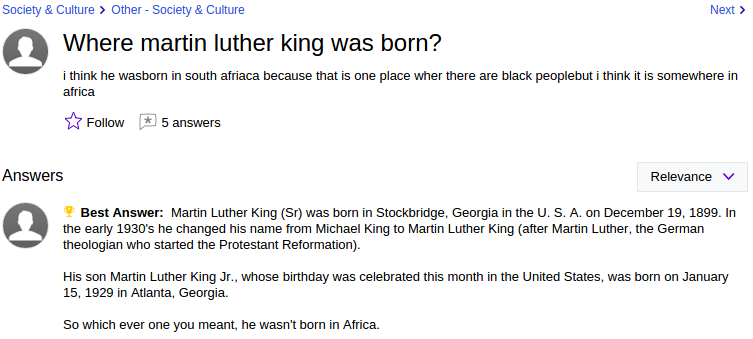
\includegraphics[width=0.5\textwidth]{img/cqa_example}
}
\caption{Example of a question and answer pair from Yahoo! Answers CQA website}
\label{figure:text2kb:cqa_example}
\end{figure}

For our experiments we use 4.4M questions from Yahoo! WebScope L6 dataset\footnote{https://webscope.sandbox.yahoo.com/}.
Question and answer texts were run through an entity linker, that detected mentions of Freebase entities.
Next, we use distant supervision assumption to label each question-answer pair with predicates between entities mentioned in the question and in the answer.
This labels are used to learn associations between question terms and predicates by computing pointwise mutual information scores (PMI) for each term-predicate pair.
Examples of scores for some terms are given in Table \ref{table:text2kb:cqa_npmi}.

\begin{table}
\centering
\begin{tabular}{| p{2cm} | p{8.5cm} | p{1cm} |}
\hline
Term & Predicate & PMI score\\
\hline
born & \texttt{people.person.date\_of\_birth} & 3.67\\
 & \texttt{people.person.date\_of\_death} & 2.73\\
 & \texttt{location.location.people\_born\_here} & 1.60\\
\hline
kill & \texttt{people.deceased\_person.cause\_of\_death} & 1.70\\
& \texttt{book.book.characters} & 1.55\\
\hline
currency & \texttt{location.country.currency\_formerly\_used} & 5.55 \\
& \texttt{location.country.currency\_used} & 3.54 \\
\hline
school & \texttt{education.school.school\_district} & 4.14 \\
& \texttt{people.education.institution} & 1.70\\
& \texttt{sports.school\_sports\_team.school} & 1.69 \\
\hline
illness & \texttt{medicine.symptom.symptom\_of} & 2.11\\
& \texttt{medicine.decease.causes} & 1.68\\
& \texttt{medicine.disease.treatments} & 1.59\\
\hline
win & \texttt{sports.sports\_team.championships} & 4.11\\
& \texttt{sports.sports\_league.championship} & 3.79\\
\hline
\end{tabular}
\caption{Examples of term-predicate pairs with high PMI scores, computed using distant supervision from a CQA collection}
\label{table:text2kb:cqa_npmi}
\end{table}

In Text2KB we evaluate candidate answer predicates by using the association (e.g., PMI) scores between predicates and the question terms (missing pairs are given a score of 0).
The minimum, average and maximum of these values are used as features to represent a candidate answer.
Such associations data can be sparse, we also use pretrained word2vec word embeddings\footnote{https://code.google.com/p/word2vec/}.
We compute predicate embeddings by taking a weighted average of term vectors from predicate's PMI table.
Each term vector is weighted by its PMI value (terms with negative score are skipped).
Then, we compute cosine similarities between predicate vector and each of the question term vectors and take their minimum, average, maximum as features.
Finally, we average embeddings of question terms and compute its cosine similarity with the predicate vector.

\textbf{Estimating Entity Associations}

A key step for ranking candidate answers is to estimate whether the question and answer entities are related in a way asked in the question.
Existing KBQA approaches usually focus on scoring the mappings between question phrases and KB concepts from a candidate SPARQL query.
However, textual data can provide another angle on the problem, as question and answer entities are likely to be mentioned together somewhere in text passages.
For example, in the bottom right corner of Figure \ref{figure:text2kb:model} we can see some passages that mention a pair of people, and the context of these mentions explains the nature of the relationships.
This data can be viewed as additional edges in a KB, which connect pairs of entities, and have associated language models, estimated from text phrases, that mention these entities.
Such edges do not have to coincide with the existing KB edges, and can connect arbitrary pairs of entities, that are mentioned together in text, therefore extending the KB.

We use the ClueWeb12 corpus with existing Freebase entity annotations and count different terms that occur in the context of a mention of a pair of different entities (we only consider mentions within 200 characters of each other).
To compute this unigram language model we use the terms separating the entities, as well as the terms within a small window (e.g., 100 characters) before and after the entity mentions.
A small sample of this data is presented in Table \ref{table:text2kb:clueweb_entitypairs_langmodel}.

\begin{table}
\centering
\begin{tabular}{| p{3.5cm} | p{3.5cm} | p{9cm} |}
\hline
Entity 1 & Entity 2 & Term counts\\
\hline
John Edwards & Rielle Hunter & campaign, affair, mistress, child, former ...\\
\hline
John Edwards & Cate Edwards & daughter, former, senator, courthouse, greensboro, eldest ...\\
\hline
John Edwards & Elizabeth Edwards & wife, hunter, campaign, affair, cancer, rielle, husband ...\\
\hline
John Edwards & Frances Quinn & daughter, john, rielle, father, child, former, paternity...\\
\hline
\end{tabular}
\caption{Example of entity pairs along with the most popular terms mentioned around the entities}
\label{table:text2kb:clueweb_entitypairs_langmodel}
\end{table}

We use this data to compute candidate ranking features as follows.
Consider question words $Q$ and an answer candidate, which contains a question entity $e_1$ and one or more answer entities $e_2$.
For each answer candidate, we compute a language model score:
$$p(Q|e_1, e_2) = \prod_{t\in Q} p(t | e_1, e_2)$$
and use the minimum, average and maximum over all answer entities as features.
To address the sparsity problem, we again use embeddings, 
\ie for each entity pair a weighted (by counts) average embedding vector of terms is computed and minimum, average and maximum cosine similarities between these vectors and question token embeddings are used as features.

\textbf{Internal text data to enrich entity representation}
In addition to external text data, many knowledge bases, including Freebase, contain text data as well, \eg Freebase includes a description paragraph from Wikipedia for many of its entities.
These text fragments provide a general description of entities, which may include information relevant to the question \cite{Sun:2015:ODQ:2736277.2741651}.
For completeness, we include them in our system as well.
Each entity description is represented by a vector of tokens, and a vector of mentioned entities.
We compute cosine similarities between token and entity vectors of the question and description of each of the answers, and use the minimum, average and maximum of the scores as features.

\subsubsection{Evaluation}
\label{section:factoid:approaches:text2kb:eval}

\begin{table*}[ht!]
\centering
\begin{tabular}{| p{5.2cm} | c | c | c | c | }
\hline
System & \centering{avg Recall} & \centering{avg Precision} & \centering{F1 of avg P and R} & avg F1 \\
\hline
OpenQA \cite{Fader:2014:OQA:2623330.2623677} & - & - & - & 0.35 \\
YodaQA \cite{baudivs2015yodaqa} & - & - & - & 0.343 \\
\hline
Jacana \cite{YaoD14} & 0.458 & 0.517 & 0.486 & 0.330\\
SemPre \cite{BerantCFL13:sempre} & 0.413 & 0.480 & 0.444 & 0.357\\
Subgraph Embeddings \cite{BordesCW14:emnlp} & - & - & 0.432 & 0.392\\
ParaSemPre \cite{BerantL14:parasempre} & 0.466 & 0.405 & 0.433 & 0.399\\
Kitt AI \cite{yao-scratch-qa-naacl2015} & 0.545 & 0.526 & 0.535 & 0.443\\
AgendaIL \cite{berant2015imitation} & 0.557 & 0.505 & 0.530 & 0.497\\
STAGG \cite{yih2014semantic} & 0.607 & 0.528 & 0.565 & 0.525\\
FMN\footnote{The model was published after the camera-ready version of our paper} \cite{jain2016question} & \textbf{0.649} & \textbf{0.552} & \textbf{0.597} & \textbf{0.557}\\
\hline
Aqqu (baseline) \cite{bastmore:cikm:2015:aquu} & 0.604 & 0.498 & 0.546 & 0.494\\
Text2KB (Wikipedia search) & \textbf{0.632}$^*$ \tiny{(+4.6\%)} & 0.498 & 0.557$^*$ \tiny{(+2.0\%)} & 0.514$^*$ \tiny{(+4.0\%)} \\
Text2KB (Web search) & \textbf{0.635}$^*$ \tiny{(+5.1\%)} & 0.506$^*$ \tiny{(+1.6\%)} & \textbf{0.563}$^*$ \tiny{(+3.1\%)} & \textbf{0.522}$^*$ \tiny{(+5.7\%)} \\
\hline
\end{tabular}
\caption{Performance of the Text2KB system on WebQuestions dataset compared to the existing approaches. The differences of scores marked * from the baseline Aqqu system are significant with p-value $<$ 0.01}
\label{table:text2kb:webquestions_results}
\end{table*}

This section reports the experimental setup, including the dataset and metrics, as well as the main methods compared for evaluating the performance of our Text2KB system. Additionally, we describe a series of ablation studies to analyze contribution of different system components.

textbf{Methods Compared}.
We compare our system, Text2KB, to state-of-the-art approaches, notably:
\begin{itemize}
\item{\textbf{Aqqu}}: a state-of-the-art baseline KBQA system~\cite{bastmore:cikm:2015:aquu}, described in Section~\ref{section:factoid:approaches:text2kb:baseline}.
\item{\textbf{Text2KB(Web search)}}: Our Text2KB system, using the Bing search engine API over the Web. 
\item{\textbf{Text2KB(Wikipedia search)}}: Our Text2KB system, using the standard Lucene search engine over the February 2016 snapshot of the English Wikipedia, in order to validate our system without the potential ``black-box'' effects of relying on a commercial Web search engine (Bing) and changing corpus (Web).
\item{\textbf{STAGG}}: One of the best current KBQA systems~\cite{yih:ACL:2015:STAGG} as measured on the WebQuestions dataset.
\end{itemize}
Additionally, other previously published results on WebQuestions are included to provide context for the improvements introduced by our Text2KB system.

\textbf{Datasets}.
We followed the standard evaluation procedure for the WebQuestions dataset, and used the original 70-30\% train-test split (3,778 training and 2,032 test instances). Within the training split, 10\% was set aside for validation to tune the model parameters and only the best-performing set of parameters selected on the validation data was used to report the results on the official test split.

\textbf{Evaluation Metrics}. 
Recent papers using the WebQuestions dataset have primarily used the average F1-score as the main evaluation metric, defined as:
$avg\ F1 = \frac{1}{|Q|} \sum_{q \in Q} f1(a^*_q, a_q)$
$$f1(a^*_q, a_q) = 2\frac{precision(a^*_q,a_q) recall(a^*_q,a_q)}{precision(a^*_q,a_q) + recall(a^*_q,a_q)}$$
$precision(a^*_q, a_q)=\frac{|a^*_q \cap a_q|}{|a_q|}$ and $recall(a^*_q, a_q) = \frac{|a^*_q \cap a_q|}{|a^*_q|}$, $a^*_q$ and $a_q$ are correct and given answers to the question q, which can be lists of entities.
Additionally, we report average precision and recall, to gain better understanding of the tradeoffs achieved by different methods.

\textbf{Main Results}.
The results of existing approaches and our Text2KB system are presented in Table \ref{table:text2kb:webquestions_results}.
We should note, that text-based QA systems typically return a ranked list of answers, whereas many answers on WebQuestions dataset are lists, which complicates the comparison between KBQA and text-based systems.
The result reported for YodaQA system is F1 score at position 1.

As we can see, Text2KB significantly improves over the baseline system and reaches the current best published result - STAGG~\cite{yih:ACL:2015:STAGG}. 
We believe that this system will also benefit from the ideas of our work.

\textbf{Datasource and Features Contribution}.
To analyze the contribution of the features and data sources we introduced, we report results from a series of ablation studies. For convenience, we introduce the following short-hand notations for different components of our system:

\begin{itemize}
\item \texttt{T} - notable type score model as a ranking feature
\item \texttt{DF} - date range filter-based query template
% \item TF - using notable type based filter
\item \texttt{WebEnt} - using web search result snippets for question entity identification
\item \texttt{WikiEnt} - using wikipedia search result snippets for question entity identification
\item \texttt{Web} - using web search results for feature generation
\item \texttt{Wiki} - using wikipedia search results for feature generation
\item \texttt{CQA} - using CQA-based \texttt{[question term, KB predicate]} PMI scores for feature generation
\item \texttt{CW} - features, computed from entity pairs language model, estimated on ClueWeb
\end{itemize}

In our results table we will use the notation \texttt{+$<$comp$>$} for a system with a certain component added, and \texttt{-$<$comp$>$} when it is removed.
For example, the baseline system will be denoted as ``\texttt{Aqqu}''.
The same system with additional date range filter query templates and notable types score model is denoted as ``\texttt{Aqqu +DF+T}'', which represents the same system as ``\texttt{Text2KB -WebEnt-Web-CQA-CL}'' (we will call it Text2KB (base)).
Our full system ``\texttt{Text2KB}'' can be also denoted as ``\texttt{Aqqu +DF+T+WebEnt+Web+CQA+CL}''.

First, we analyze the improvements introduced by different components of our system (Table \ref{table:text2kb:ablation:entities_vs_features}).
As we can see, additional date range filters and notable types model (\texttt{Aqqu+DF+T}) are responsible for an increased recall and a drop in precision compared to the baseline model.
Features generated from Wikipedia search results, CQA data and ClueWeb entity pair language models (\texttt{+Wiki+CQA+CL}) improve average F1 by 0.007 (+1.4\%) compared to the base model, adding entity linking using Wikipedia search results improves results even more (+3\%).

Web search results (\texttt{+Web+CQA+CL}) turned out to be more helpful than Wikipedia results (\texttt{+Wiki+CQA+CL}), which is natural since Wikipedia is a subset of the web.
This was one of the reasons we didn't combine Wikipedia and Web search together.
Finally, entity linking and all text-based features combined achieves an even higher score, proving that their contributions are independent.

We now anylize the contribution of the different data sources.
We will remove a group of web search, CQA or Clueweb-based features and see how the performance of the whole system changes (Table \ref{table:text2kb:ablation:features}).
As we can see, all data sources have an impact on the system performance, and web search results based features provide the most useful signal for answer ranking.

Figure \ref{figure:text2kb:feature_importances} plots a subset of features ranked by their Gini index-based importance scores.
The figure supports the observation that web search results features are the most useful, however, other text data sources also contribute to the improvement.

\begin{table}[h]
\centering
\begin{tabular}{| p{6cm} | c | c | c | }
\hline
System & R & P & F1 \\
\hline
\texttt{Aqqu} & 0.604 & 0.498 & 0.494\\
\texttt{Text2KB (base) = Aqqu+DF+T} & 0.617 & 0.481 & 0.499 \\
\hline
\texttt{+Wiki+CQA+CL} & 0.623 & 0.487 & 0.506 \\
\texttt{+WikiEnt +Wiki+CQA+CL} & 0.632 & 0.498 & 0.514 \\
\hline
\texttt{+WebEnt} & 0.627 & 0.492 & 0.508 \\
\texttt{+Web+CQA+CL} & 0.634 & 0.497 & 0.514 \\
\texttt{+WebEnt +Web+CQA+CL} & 0.635 & 0.506 & 0.522 \\
\hline
\end{tabular}
\caption{Average Recall (R), Precision (P), and F1 of Aqqu and Text2KB system with and without different components. +A means that a component A is added to the Text2KB (base) system.}
\label{table:text2kb:ablation:entities_vs_features}
\end{table}

\begin{table}[h]
\centering
\begin{tabular}{| p{6cm} | c | c | c | }
\hline
System & R & P &  F1 \\
\hline
Text2KB (Web search) & 0.635 & 0.506 & 0.522 \\
\hline
% THIS PART ANSWERS HOW GOOD ARE EACH OF THE PROPOSED DATASETS
% extent_cqa_clueweb_dates_typemodel_rf100.log : -web
\texttt{Text2KB -Web} & 0.633 & 0.496 & 0.513 \\
% extent_web_clueweb_dates_typemodel_rf100.log : -cqa
\texttt{Text2KB -CQA} & 0.642 & 0.499 & 0.519 \\
% extent_web_cqa_dates_typemodel_rf100.log : -clueweb
\texttt{Text2KB -CL} & 0.644 & 0.505 & 0.523 \\
\hline
% extent_web_dates_typemodel_rf100.log : -clueweb-cqa
\texttt{Text2KB -CQA-CL} & 0.642 & 0.503 & 0.522 \\
% extent_clue_dates_typemodel_rf100.log : -web-cqa
\texttt{Text2KB -Web-CQA} & 0.631 & 0.498 & 0.514 \\
% extent_cqa_dates_typemodel_rf100.log : -web-clueweb
\texttt{Text2KB -Web-CL} & 0.622 & 0.493 & 0.508 \\
%\hline
% extent_web_cqa_clueweb_dates_types_typemodel_rf100.log : everything, including type filters
%\texttt{Text2KB} & 0.6354 & 0.5059 & 0.5223 \\
\hline
\end{tabular}
\caption{Average Recall (R), Precision (P), and F1 of Text2KB with and without features based on web search results, CQA data and ClueWeb collection.}
\label{table:text2kb:ablation:features}
\end{table}

\begin{figure*}
\centering
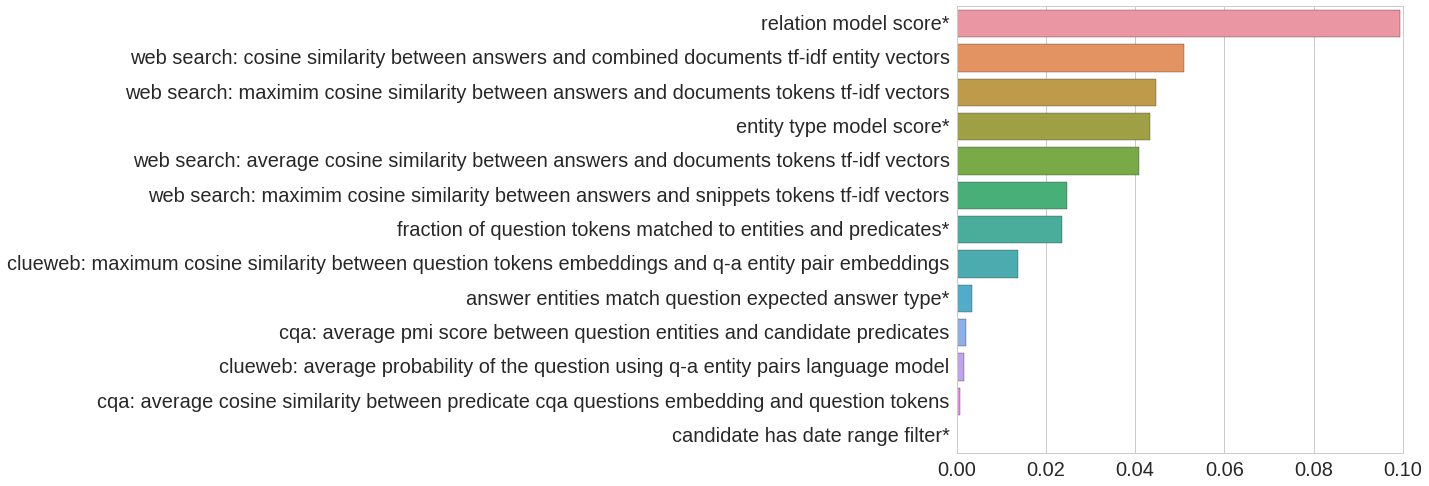
\includegraphics[width=\textwidth]{img/feature_importances}
\caption{A plot of Gini importances of different features of our answer ranking random forest model (features marked * are not text-based and are provided for comparison)}
\label{figure:text2kb:feature_importances}
\end{figure*}

In summary, Text2KB significantly outperforms the baseline system, and each of the introduced components contributes to this improvement.
Web search results data turned out to be the most useful resource, and it significantly improves the quality by helping with question entity identification and candidate ranking.
Next, we analyze the system performance in more detail, and investigate factors for future extension.

\subsubsection{Analysis}
\label{section:factoid:approaches:text2kb:analysis}

We now investigate how our system would compare to other systems on the same benchmark; then, we investigate in depth the different error modes, which helps identify the areas of most substantial future improvements.

We took an existing KBQA systems and demonstrated that by combining evidence from knowledge base and external text resources we can boost the performance.
A reasonable question is whether the same approach will be helpful to other systems, \eg the currently best system -- STAGG~\cite{yih:ACL:2015:STAGG}.
STAGG differs from our baseline system Aqqu in the components: entity linking algorithm, a set of query templates and ranking methods.
Therefore, our approach is complementary and should be helpful for STAGG as well.
To support this claim, we made an experiment to combine answers of STAGG and Text2KB.
One of the advantages of the former is its set of filters, that restricts list results to entities of certain type, gender, \etc
Therefore, we combined answers of STAGG and Text2KB using a simple heuristic: we chose to use the answer returned by STAGG if the number of answer entities is less than in the Text2KB answer, otherwise we use the answer of our approach.
Table \ref{table:text2kb:combine_stagg} gives the results of the experiment, and as we can see the combination achieves a slightly better average F1 score.
Alternatively, we can look at the Oracle combination of the systems, which always selects the answer with the higher F1.
As we can see such a combination results in a performance of 0.606, which is much higher than either of the systems.

\begin{table}
\centering
\begin{tabular}{| p{6cm} | c | }
\hline
System  & avg F1 \\
\hline
Text2KB & 0.522\\
\hline
STAGG~\cite{yih:ACL:2015:STAGG} & 0.525\\
Text2KB + STAGG & 0.532 (+1.3 \%) \\
Text2KB + STAGG (Oracle) & 0.606 (+15.4 \%) \\
\hline
\end{tabular}
\caption{Average F1 for combinations of Text2KB and STAGG using a simple heuristic based on the length of the answer list and Oracle upper bound}
\label{table:text2kb:combine_stagg}
\end{table}

As we mentioned earlier, answers to 112 of the test questions in the WebQuestions dataset involve predicates that weren't observed in the training set, which may be a problem for approaches that rely on a trained lexicon.
We evaluated both systems on these questions, and indeed the performance is very low, \ie the average F1 score of Text2KB is 0.1640 compared to 0.1199 for STAGG\footnote{Unfortunately, the number of questions is too low to show statistical significance (p-value=0.16) of the difference}.

\begin{figure}
\centering
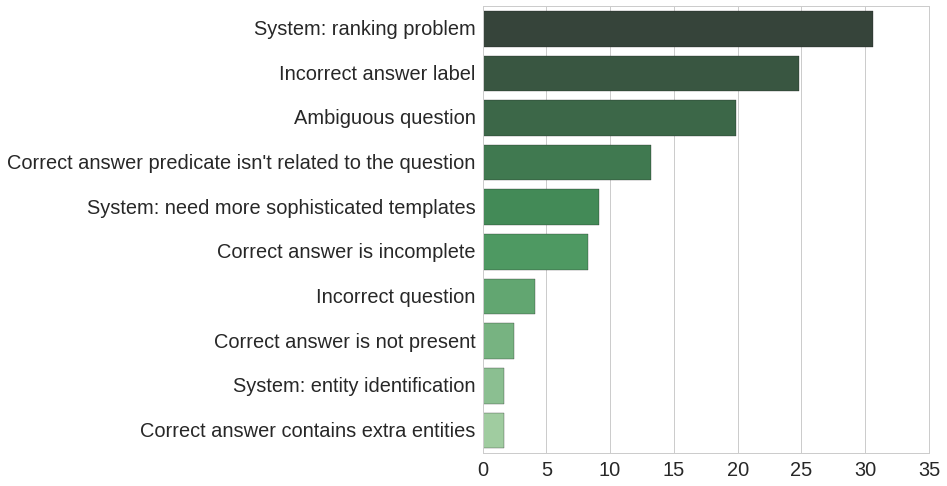
\includegraphics[width=0.6\textwidth]{img/error_analysis}
\caption{Distribution of problems with questions, where Text2KB returns an answer with F1$<$1}
\label{figure:text2kb:error_analysis}
\end{figure}

To get a better insights into the problems that remain, we collected 1219 questions for which Text2KB didn't return completely correct answer, \ie F1 score $<$ 1.
We manually looked through a couple of hundreds of these examples and grouped the problems into several clusters (Figure \ref{figure:text2kb:error_analysis}).

As we can see candidate ranking is still the major problem, and it accounts for $\sim31\%$ of the cases.
The second problem is incorrect ground truth labels (almost 25\% of reported errors).
Another set of questions has incomplete or overcomplete ground truth answer list.
Typical examples are questions asking for a list of movies, books, landmarks, \etc
The ground truth answer usually contains $\sim10$ entities, whereas the full list is often much larger.
This seems to be an artifact of the labeling process, where the answer was selected from the Freebase entity profile page, which shows only a sample of 10 entities, while the rest are hidden behind the ``N values total'' link.
About 20\% of the questions are ambiguous, \ie questions have no strict 1-1 correspondence with any of the predicates and can be answered by multiple ones without any obvious preferences.
For example, the question \textit{``what did hayes do?''} can be answered by profession, occupied position or some other achievements.
Another problem is when there is no predicate that answers the question.
For example, the question \textit{``what do people in france like to do for fun?''} doesn't have a good match among the facts stored in Freebase.
The ground truth entity \texttt{Cycling} comes from the list Olympic sport competitions country participated\footnote{\texttt{olympics.olympic\_participating\_country.athletes}}.

Text2KB components were quite effective in resolving some of the problems.
Web search results helped identify the right question topical entity in a number of cases, \eg \textit{``what did romo do?''} mentions only the last name of the Dallas Cowboys quarterback and the baseline system were unable to map it to the right entity.
Web search results provides more than enough evidence that ``\textit{romo}'' refers to \texttt{Tony Romo}.
However, there are a number of loses, introduced by added unrelated entities.
For example, the entity \texttt{I Love Lucy} was added for the question \textit{``what was lucille ball?''}, because the term \textit{lucy} had high similarity with \textit{lucille}.
A portion of these problems can be fixed by a better entity linking strategy, \eg \cite{SMAPH_ERD:2014}.
An interesting example, when external text resources improved the performance is the question \textit{``what ship did darwin sail around the world?''}.
This is actually a hard question, because the ship entity is connected to the \texttt{Charles Darwin} entity through the ``knownFor'' predicate along with some other entities like \texttt{Natural selection}.
% \footnote{\texttt{user.lindenb.default\_domain.scientist.known\_for}
Thus, the predicate itself isn't related to the question, but nevertheless, the name of the ship \texttt{HMS Beagle} is mentioned multiple times in the web search results, and entity pair model computed from ClueWeb also has high scores for the terms ``ship'' and ``world''.

There are several major reasons for the loses, introduced by features based on external text resources.
Some entities often mentioned together and therefore one of them gets high values of cooccurrence features.
For example, the baseline system answered the question \textit{``when did tony romo got drafted?''} correctly, but since \texttt{Tony Romo} is often followed by \texttt{Dallas Cowboys}, Text2KB ranked the team name higher.
Another common problem with our features is an artifact of entity linking, which works better for names and often skips abstract entities, like professions.
For example, the correct answer to the question \textit{``what did jesse owens won?''} is an entity with the name \texttt{Associated Press Male Athlete of the Year}, which is rarely mentioned or it's hard to find such mentions.
Some problems were introduced by a combination of components.
For example, for \textit{``where buddha come from?''} a topical entity \texttt{Buddhism} was introduced from search results, and it generated \texttt{Gautama Buddha} as one of the answer candidates.
This answer was ranked the highest due to large number of mentions in the search results.

\subsubsection{Summary}
\label{section:factoid:approaches:text2kb:summary}

In summary, in this section we demonstrated that unstructured text resources can be effectively utilized for knowledge base question answering to improve query understanding, candidate answer generation and ranking.
Textual resources can help KBQA system mitigate the problems of matching between knowledge base entities and predicates and textual representation of the question.

Unfortunately, Text2KB doesn't help with the problem of knowledge base incompleteness, \ie our system won't be able to respond to the question, which refers to an entity, a predicate or a fact, which is missing in a KB.
Section~\ref{section:factoid:proposal} describes research I propose to overcome this problem.

% =-=-=-=-=-=-=-=-=-=-=-=-=-=-Text2KB: End=-=-=-=-=-=-=-=-=-=-=-=-=-=-=-=-=-

\section{Proposed Research: Hybrid Question Answering using Text and Knowledge Base Data}
\label{section:factoid:proposal}

Experiments from Section~\ref{section:factoid:approaches:text2kb} demonstrated the effectiveness of unstructured data, such as natural language text, to bridge the lexical chasm between KB concepts and natural language questions.
However, such an approach only works if concepts and facts referred in the question actually exists in KB.
In reality, a big fraction of real user questions cannot be answered using KB data, which is supported by relatively low performance of KBQA systems on general set of factoid questions, such as TREC QA \cite{Sun:2015:ODQ:2736277.2741651}.



\subsection{Method}
\label{section:factoid:proposal:method}

\begin{figure}
\centering
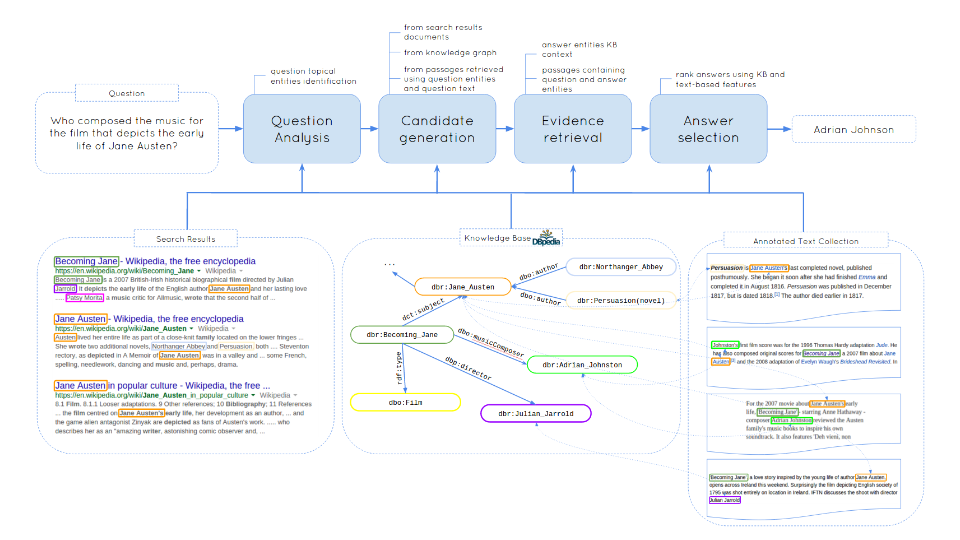
\includegraphics[width=\textwidth]{img/text_and_kb}
\caption{Architecture of a hybrid factoid question answering system, that uses a combination of structured knowledge base and unstructured text data}
\label{figure:factoid:text_kb}
\end{figure}

In this section I propose a novel hybrid QA architecture, that combines unstructured text and structured knowledge base data for joint inference.
Figure \ref{figure:factoid:text_kb} gives a general overview of the proposed system.
The idea is to extend the documents representation with annotations of KB entity mentions, which essentially creates additional edges in the knowledge graph.
These edges connecting KB entities with text fragments can be traversed by a QA system in both directions in order to get more syntactic (from entity to text) or semantic (from text to entity) information.
In addition, text fragments, that mention 2 different entities close to each other can serve as an addition knowledge triple.
Unlike information extraction approaches, however, we don't try to extract the predicate and get rid of all the other information stated in a sentence.
In the proposed approach we are going to use text similarity metrics to retrieve such triples.

The main stages of the proposed QA pipeline are the following (Figure~\ref{figure:factoid:text_kb}):
\begin{enumerate}
\item \textbf{Question analysis}
	\begin{itemize}
	  \item \textbf{Pre-processing}: identify mentions of KB entities in text document collection and index the documents text and mentions in separate fields
  	  \item \textbf{Topical entity identification}: search the text collection using question (or reformulated question \cite{AgichteinLG01}) as a query and use an approach similar to \cite{cornolti2014smaph} to detect question topical entities
    \end{itemize}
  
\item \textbf{Candidate generation}
	\begin{itemize}
	  \item \textbf{Candidate generation from text}: extract candidate answer (or intermediate answer) entities with evidence from the retrieved text documents using existing techniques, e.g. \cite{tsai2015web}.
  	  \item \textbf{Candidate generation from KB}: explore the KB neighborhood of question topical entities and entities extracted from text documents on the previous step
	  \item \textbf{Candidate generation from KB \& Text}: use entity and text index to find entities mentioned near question topical entity and question terms in the document collection
	\end{itemize}
\item \textbf{Evidence retrieval}
    \begin{itemize}
	  \item \textbf{KB evidence extraction}: match neighborhood of answer entities (entity type and other entities) against the question to get additional evidence
      \item \textbf{Text evidence extraction}: estimate the similarity between the collection text fragments mentioning question and answer entities and the question text
    \end{itemize}
\item \textbf{Answer selection}
	\begin{itemize}
	  \item \textbf{Rank candidate}: rank candidate answers using evidence extracted from the KB as well as from text. One particular appealing idea for a ranking model is to estimate $p(q|G_e)$, where $G_e$ is a knowledge subgraph, associated with the current answer candidate. This probability estimates how likely the question could be generated from the knowledge subgraph language model.
    \end{itemize}
\end{enumerate}

As a motivating example, let's consider the following question from the QALD dataset: ``\textit{Who composed the music for the film that depicted the early life of Jane Austen?}''.
Even though it's quite easy to identify the ``\texttt{Jane Austen}'' entity in the question, the knowledge base (dbPedia in this example) cannot help us to determine which movie is being referred to.
However, there are plentiful of documents on the web, that describe the plot of the \texttt{Becoming Jane} movie, and a system can use the proximity of terms from the question \textit{``... depicted early life of Jane Austen''} to the movie entity.
Unfortunately, extracting the name of the composer from these documents is quite challenging, but this task can be easily accomplished by checking the value of the \texttt{musicComposer} property in the knowledge base.
At the end, for each candidate answer entity, we have all the KB information and passages that mention this entity as evidence to help with the correct answer selection.

Essentially, the proposed model is a search based approach, similar to existing information extraction methods for knowledge base question answering~\cite{YaoD14,bastmore:cikm:2015:aquu}, but over the knowledge graph extended with the links to entity mentions in text collections.
In traditional KBQA a special lexicon is used to match terms and phrases in the question to predicates, which essentially represent KB edges.
For text edges I'm planning to use the following two approaches: IR-based methods, in particular recent advances in entity search~\cite{zhiltsov2015fielded,nikolaev2016parameterized}, and neural network joint embeddings of predicates and text fragments~\cite{BordesCW14:emnlp,miller2016key}.

\subsection{Experimentation}
\label{section:factoid:proposal:experiments}

To evaluate the performance of the proposed approach I will compare it against several alternatives on multiple datasets.
The baselines I will compare against include knowledge base question answering system Aqqu~\cite{bastmore:cikm:2015:aquu}, a semantically enriched text-based system QuASE~\cite{Sun:2015:ODQ:2736277.2741651}, a hybrid YodaQA system, designed to be an open source analogue to IBM Watson~\cite{baudivs2015yodaqa} and open question answering approach of A.Fader et al~\cite{Fader:2014:OQA:2623330.2623677}.

Most of the recent works in knowledge base question answering were evaluated on the WebQuestions dataset~\cite{BerantCFL13:sempre}.
This dataset was recently updated to include ground truth semantic parses and many wrong labels were fixed~\cite{yih2016webquestionssp}.
I'm planning to evaluate the system I'm going to built on these datasets.
Since the answers to these questions can be lists, the official evaluation metric is average F1 score over all questions.
However, WebQuestions dataset has its limitations, \eg all the questions are selected so that they could be answered from Freebase.
Furthermore, answers to the question were labeled using entities' Freebase profile pages, which only displays relations in the close proximity to the target entity.
This makes it possible to exploit a small set of templates to generate candidate answer queries.

Traditionally, most of the works in question answering have been evaluated on the TREC QA datasets.
These datasets come with a set of regular expression patterns that can judge an answer as correct or incorrect.
Unfortunately, these patterns aren't complete and researchers often end up re-validating the answers of their systems manually~\cite{Sun:2015:ODQ:2736277.2741651,tsai2015web}.
Unlike most of the previous approaches, however, the proposed system aims at retrieving KB entities as answers of the questions.
Therefore, I will annotate TREC QA datasets with KB entity identifiers of the correct answers.
The baseline systems I mentioned were evaluated of some parts of TREC QA dataset, and I'm going to use reported results instead of reimplementing them.
For my system, I will use ClueWeb12 collection, which was annotated with Freebase entity mentions~\cite{gabrilovich2013facc1}.
The text around mentions will be indexed with Lucene\footnote{https://lucene.apache.org/} open source search engine.
The metrics used for evaluation typically include accuracy and mean reciprocal rank (MRR).

However, TREC QA dataset contains only a couple of thousands of examples, which is relatively small.
As an alternative, I'm designing a new factoid QA dataset, derived from questions posted to Yahoo! Answers CQA website.


\subsubsection{New factoid question answering dataset}
\label{section:factoid:proposal:experiments:dataset}

% \todo{Note to myself: I guess we won't be allowed to make this dataset public as is, because it's derived from Yahoo WebScope dataset.}

Community question answering websites contains hundreds of millions of different questions and corresponding answers, posted by real users.
A fraction of these questions represent factoid information needs.
I'm going to filter a subset of these questions using a set of heuristics or rules.
For example, we can select a subset of QnA pairs with at least one entity in the question and answer, without personal pronouns, words like ``\textit{recommend}'', ``\textit{suggest}'', superlative adjectives like ``\textit{best}'', \etc.
Next this QnA pairs will be further labeled by Mechanical Turk users, who will determine if the questions are indeed factoid and non-subjective and select the actual answer entity from the list of entities, mentioned in the answer text.
The preliminary analysis showed, that from 3.8M QnA pairs from Yahoo! Answers WebScope collection, 80K passed the heuristics filters described above and about 30\% of them are actually good factoid questions.
Examples of questions are: ``\textit{What was James Bond's wife's name?}'', ``\textit{What is the name of the second US astronaut to land on the moon?}'', ``\textit{When was the first "cartoon human" movie?}'', ``\textit{What movie did Joe Pesci describe kids as "YUTS"?}''.
I expect this dataset to contain ~10K real user questions annotated with answer entities, which can be used for future research in question answering in both knowledge base and general factoid question answering.

In my thesis this dataset will be used to further compare performances of the proposed approach versus existing KBQA, text and hybrid systems with open code.

\section{Summary}
\label{section:factoid:summary}

In this section we considered two different ways of combining unstructured and structured data to improve factoid question answering.
Relation extraction from question-answer pairs aims at filling some gaps in KB fact coverage, whereas semantic annotations of text documents provides a way to incorporate information available in unstructured text documents for reasoning along with KB data to improve the performance of factoid question answering.
The experiments proposed in this Chapter will help to answer the question on whether combining structured and unstructured data into a single entity graph is beneficial for the question answering performance compared to text-based, KBQA-based or alternative hybrid approaches.

Factoid questions represent just a part of user information needs. Many problems require more elaborate response, such as a sentence, list of instructions or, in general, a passage of text.
Such questions are usually referred to as non-factoid questions and they will be the focus of the Chapter~\ref{chapter:non-factoid}.